% state/pose2.tex

\chapter{Pose2}

The first canonical state layer in AIM is \(\mathrm{pose2}\). It provides
the minimal intrinsic reconstruction state of an alignment and serves
as the canonical home for planar geometry. The chapter therefore treats
pose2 as the persistent intrinsic state from which higher-level spatial
and operational states are derived, rather than as an auxiliary
geometric convenience.

% ============================================================
\section{Definition of pose2}
% ============================================================

\begin{definition}[pose2]
A planar pose state at arc-length position \(s\) is defined as
\[
\mathrm{pose2}(s)
=
\bigl(
\gamma(s),
\theta(s)
\bigr).
\]
\label{def:pose2}
\end{definition}

This state records the intrinsic planar position \(\gamma(s)\) and the
intrinsic tangent orientation \(\theta(s)\). The canonical pose2 system
is the planar reconstruction system in \cref{eq:pose2-system}.

% ============================================================
\section{Curvature-Driven Reconstruction}
% ============================================================

\begin{principle}[Curvature-driven reconstruction]
Within AIM, planar geometry is reconstructed intrinsically from
curvature evolution.
\end{principle}

The intrinsic reconstruction chain follows directly from
\cref{eq:curvature-relation,eq:state-evolution,eq:planar-tangent}.
Position and orientation therefore do not appear as independently stored
geometric primitives. They emerge through integration of curvature along
arc length.

The figure below answers the local engineering question for this
section: which quantities are primary in reconstruction, and which are
derived runtime consequences of that primary law?

\begin{figure}[ht]
\centering

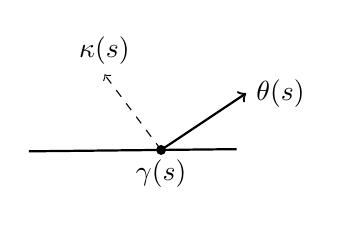
\begin{tikzpicture}[scale=1.2]

% Curve
\draw[thick, domain=0:2.2, samples=50]
plot ({\x}, {0.4*sin(1.5*\x)});

% Point
\coordinate (P) at (1.4,{0.4*sin(1.5*1.4)});
\fill (P) circle (1.5pt);

% Tangent
\draw[->, thick]
(P) -- ++(0.9,{0.4*cos(1.5*1.4)*1.5})
node[right] {$\theta(s)$};

% Curvature hint
\draw[->, dashed]
(P) -- ++({-0.4*cos(1.5*1.4)*1.5},0.8)
node[above] {$\kappa(s)$};

% Label
\node[below] at (P) {$\gamma(s)$};

\end{tikzpicture}

\caption{
Planar geometry emerges through intrinsic curvature-driven
reconstruction.
Within AIM, curvature is treated as the primary geometric quantity.
}
\label{fig:pose2-curvature-reconstruction}
\end{figure}

The interpretation is direct: \(\kappa(s)\) drives tangent evolution,
and tangent evolution drives positional reconstruction. The engineering
consequence is that persistent storage should prioritize intrinsic
curvature semantics, while pose coordinates remain reconstructable
derived state.

% ============================================================
\section{Initial Conditions}
% ============================================================

\begin{definition}[Initial pose2 state]
A pose2 trajectory is uniquely determined by:
\[
\gamma(0),
\qquad
\theta(0),
\]
together with the curvature law
\[
\kappa(s).
\]
\label{def:initial-pose2}
\end{definition}

The curvature law acts as the geometric control function of planar state
evolution. In this sense, pose2 is a reconstruction state governed by an
intrinsic control law rather than by a stored geometric coordinate list.

% ============================================================
\section{Pose2 as Persistent Kernel}
% ============================================================

\begin{proposition}
Within AIM, pose2 forms the persistent intrinsic reconstruction kernel
of the alignment model.
\label{prop:pose2-persistent-kernel}
\end{proposition}

Pose2 is sufficient for persistent planar reconstruction of intrinsic
alignment geometry. Higher-level geometric and operational quantities
are derived from pose2 rather than stored redundantly.

% ============================================================
\section{Connection to Sparse Alignment}
% ============================================================

Within the sparse alignment model, \(\mathrm{cGeom}\) elements are
interpreted as local curvature operators contributing to reconstruction
of the global pose2 trajectory. Fixed and transition elements therefore
do not primarily store geometry itself, but rules governing geometric
evolution. The sparse alignment model can thus be read as a compact
integration program for reconstructing pose2 trajectories.

% ============================================================
\section{Intrinsic Interpretation}
% ============================================================

Pose2 separates intrinsic geometric behaviour from derived geometric
quantities. Curvature acts as the intrinsic control quantity, whereas
position and orientation emerge through reconstruction. This separation
is one of the central structural principles of the AIM framework.

% ============================================================
\section{Relation to pose3}
% ============================================================

Within AIM, pose2 forms the persistent intrinsic reconstruction kernel,
whereas pose3 represents an extended runtime-evaluated spatial state.
pose3 is derived dynamically from pose2 reconstruction together with
profile evaluation, cant evaluation, frame construction, and runtime
coordinate services. This separation avoids redundancy and
synchronization instability between planar, cant, profile, and runtime
representations.

% ============================================================
\section{Canonical Interpretation}
% ============================================================

\begin{proposition}
Within AIM, intrinsic railway geometry is fundamentally curvature-driven.
\end{proposition}

\begin{proposition}
pose2 represents the canonical persistent intrinsic geometry state from
which higher-level runtime states are derived.
\end{proposition}

% ============================================================
\section{Connection to AIM}
% ============================================================

\begin{summary}
pose2 is the fundamental intrinsic planar state representation of
railway alignment.

Within AIM, pose2 forms the persistent reconstruction kernel from which
planar geometry is generated through curvature-driven integration.

Higher-dimensional runtime states such as pose3 are derived dynamically
from this kernel together with cant, profile, frame, and runtime
evaluation services.
\end{summary}
